\chapter{Khúc xạ ánh sáng}
\section{Lý thuyết trọng tâm}
\subsection{Hiện tượng khúc xạ ánh sáng}
Khúc xạ ánh sáng là hiện tượng lệch phương (gãy) của các tia sáng khi truyền xiên góc qua mặt phân cách giữa hai môi trường trong suốt khác nhau.
\subsection{Định luật khúc xạ ánh sáng}
\begin{center}
	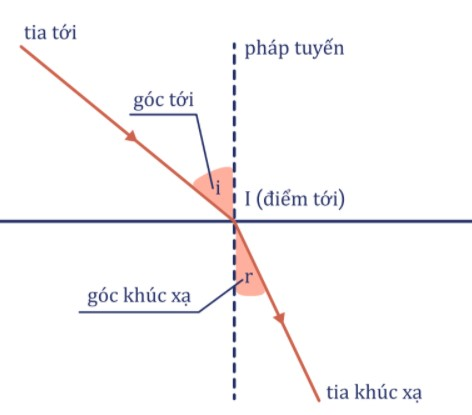
\includegraphics[scale=0.8]{../figs/VN11-PH-34-L-023-1-h57.jpg}
\end{center}
\begin{itemize}
	\item Tia khúc xạ nằm trong mặt phẳng tới (tạo bởi tia tới và pháp tuyến) và ở phía bên kia pháp tuyến so với tia tới.
	\item Với hai môi trường trong suốt nhất định, tỉ số giữa sin góc tới $(\sin i)$ và sin góc khúc xạ $(\sin r)$ luôn luôn không đổi: 
	\begin{equation}
	\dfrac{\sin i}{\sin r}=\dfrac{n_2}{n_1},
	\end{equation}
	Công thức được viết dưới dạng đối xứng: 
	\begin{equation}
	n_1\cdot \sin i=n_2\cdot \sin r,
	\end{equation}
	trong đó:
	\begin{itemize}
		\item $i$ là góc tới,
		\item $r$ là góc khúc xạ,
		\item $n_1$ là chiết suất của môi trường tới,
		\item $n_2$ là chiết suất môi trường khúc xạ. 
	\end{itemize}
\end{itemize}
\section{Bài tập }
\begin{dang}{Công thức định luật khúc xạ ánh sáng}
\end{dang}
\textbf{Phương pháp giải}

Sử dụng công thức định luật khúc xạ ánh sáng:
\begin{equation}
n_1\cdot \sin i=n_2\cdot \sin r,
\end{equation}

Góc lệch giữa tia tới và tia khúc xạ 
	\begin{equation}
		D=|i-r|.
	\end{equation} 

\vspace{1em}
\viduii{2}{
Tia sáng đi từ nước có chiết suất $n_1=\dfrac{4}{3}$ sang thủy tinh có chiết suất $n_2=\text{1,5}$. Tính góc khúc xạ và góc lệch $D$ tạo bởi tia khúc xạ và tia tới, biết góc tới $i=30^\circ$. 
\begin{mcq}(2)
	\item $r=\text{24,4}^\circ$, $D=\text{5,6}^\circ$.
	\item $r=\text{26,4}^\circ$, $D=\text{3,6}^\circ$.
	\item $r=\text{28,4}^\circ$, $D=\text{1,6}^\circ$.
	\item $r=\text{29,4}^\circ$, $D=\text{0,6}^\circ$.
\end{mcq}}
{\begin{center}
	\textbf{Hướng dẫn giải:}
\end{center}

{Công thức định luật khúc xạ ánh sáng:
	$n_1\sin i=n_2\sin r$
	
	$\Rightarrow \sin r=\dfrac{n_1\sin i}{n_2}=\dfrac{4}{9}$
	
	$\Rightarrow r= \text{26,4}^\circ$.

Góc lệch $D=|i-r|=\text{3,6}^\circ$.

\textbf{	Đáp án: B.}
}
}

\viduii{2}{
Tia sáng truyền trong không khí tới gặp mặt thoáng của chất lỏng có chiết suất bằng $\sqrt{3}$. Ta được hai tia phản xạ và khúc xạ vuông góc với nhau. Tính góc tới.

\begin{mcq}(4)
	\item $\dfrac{\pi}{6}$.
	\item $\dfrac{\pi}{4}$.
	\item $\dfrac{\pi}{3}$.
	\item $\dfrac{\pi}{2}$
\end{mcq}}{
\begin{center}
	\textbf{Hướng dẫn giải:}
\end{center}

{
Công thức định luật khúc xạ ánh sáng:	$n_1\cdot \sin i=n_2\cdot \sin r$.

Do $n_1=1, n_2=\sqrt{3}$ nên $\dfrac{\sin i}{\sin r}=n_2$.

Theo định luật phản xạ ánh sáng, góc tới $i$ bằng góc phản xạ $i'$.

Vì $i'+r=i+r=\dfrac{\pi}{2}\Rightarrow \sin r=\sin \left( \dfrac{\pi}{2}-i\right)=\cos i$.

$\Rightarrow \dfrac{\sin i}{\sin r}=\dfrac{\sin i}{\cos i}=\tan i=n_2=\sqrt{3}\Rightarrow i=\dfrac{\pi}{3}$.
	
\textbf{	Đáp án: C.}
	}}

\viduii{3}{

Ba môi trường trong suốt (1), (2), (3) có thể đặt tiếp giáp nhau. Với cùng góc tới $60^\circ$; nếu ánh sáng truyền từ (1) vào (2) thì góc khúc xạ là $45^\circ$; nếu ánh sáng truyền từ (1) vào (3) thì góc khúc xạ là $30^\circ$. Nếu ánh sáng truyền từ (2) vào (3) vẫn với góc tới $60^\circ$ thì góc khúc xạ là

\begin{mcq}(4)
	\item $18^\circ$.
	\item $28^\circ$.
	\item $38^\circ$.
	\item $48^\circ$.
\end{mcq}}{
\begin{center}
	\textbf{Hướng dẫn giải:}

\end{center}
{
	
	Khi ánh sáng đi từ môi trường (1) sang môi trường (2): $\dfrac{\sin 45^\circ }{\sin 60^\circ}=\dfrac{n_2}{n_1}$.
	
	Khi ánh sáng đi từ môi trường (1) sang môi trường (3): $\dfrac{\sin 60^\circ }{\sin 30^\circ}=\dfrac{n_3}{n_1}$.
	
	Suy ra:  $\dfrac{\sin 45^\circ }{\sin 30^\circ}=\dfrac{n_3}{n_2}$ (*)
	
	Khi ánh sáng đi từ môi trường (2) sang môi trường (3): $\dfrac{\sin 60^\circ }{\sin r}=\dfrac{n_3}{n_2}$ (**)
	
	Từ phương trình (*) và (**), suy ra: $\dfrac{\sin 60^\circ }{\sin r}=\dfrac{\sin 45^\circ }{\sin 30^\circ}\Rightarrow r=38^\circ$.
		
\textbf{	Đáp án: C.}
}}

\begin{dang}{Bài toán tìm chiều sâu của lớp nước}
\end{dang}
\textbf{Phương pháp giải}

Công thức định luật khúc xạ ánh sáng:
\begin{equation}
n_1\cdot \sin i=n_2\cdot \sin r,
\end{equation}

Góc lệch giữa tia tới và tia khúc xạ $D=|i-r|$. 

Sử dụng các công thức lượng giác giác như $\sin, \ \cos, \ \tan,..$,  các tính chất hình học của tam giác đồng dạng, tam giác vuông, cân,...
\vspace{1em}

\vidu{3}{
Một cây cọc dài được cắm thẳng đứng xuống một bể nước chiết suất $n=\dfrac{4}{3}$. Phần cọc nhô ra ngoài mặt nước là 30 cm, bóng của nó trên mặt nước dài 40 cm và dưới đáy bể nước dài 190 cm. Tính chiều sâu của lớp nước. 
\begin{center}
	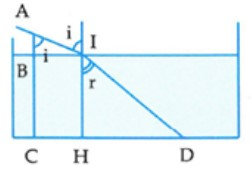
\includegraphics[scale=0.8]{../figs/VN11-PH-34-L-023-1-h58.jpg}
\end{center}
\begin{mcq}(4)
	\item $100\ \text{cm}$.
	\item $300\ \text{cm}$.
	\item $400\ \text{cm}$.
	\item $200\ \text{cm}$.
\end{mcq}}{
\begin{center}
	\textbf{Hướng dẫn giải:}
\end{center}

{Ta có: $\tan i=\dfrac{\text{BI}}{\text{AB}}=\dfrac{40}{3}\Rightarrow i=\text{53}^\circ$.
	
	
	Công thức định luật khúc xạ ánh sáng:
	$n_1\sin i=n_2\sin r$
	
	$\Rightarrow \sin r=\dfrac{n_1\sin i}{n_2}=\dfrac{4}{9}\Rightarrow r= \text{26,4}^\circ$.
	
	Công thức định luật khúc xạ ánh sáng: $\dfrac{\sin i}{\sin r}=n\Rightarrow \sin r=\dfrac{\sin i}{n}=\text{0,6}\Rightarrow r=37^\circ$.
	
	$\tan r=\dfrac{\text{HD}}{\text{IH}}=\dfrac{\text{CD}-\text{CH}}{\text{AB}}\Rightarrow \text{IH}=\dfrac{\text{CD}-\text{CH}}{\tan r}$.

Ta thay các đoạn $\text{CD}=120\ \text{cm}, \ \text{CH}=140\ \text{cm}, \ \tan r=\text{0,75}$.

Suy ra $\text{IH}=\text{200}\ \text{cm}$.

		
\textbf{	Đáp án: D.}
}}

